\chapter{Evaluation}
\label{chap:evaluation}
In this chapter, we aim to evaluate different aspects of the developed system. Section \ref{sec:cost_and_performance} shows a cost as well as a performance analysis of the developed \gls{sc}. Section \ref{sec:field_test} concludes the analyses with a field test of a simulated artwork transportation scenario. Finally, this chapter is concluded with a discussion in Section \ref{sec:eval_discussion} To evaluate the performance of the system we also recorded the response time of each request. This can give an indicator

\section{Cost and Performance Analysis}
\label{sec:cost_and_performance}
The primary cost factor of the artis-system is the \gls{sc}. Each execution of a function that mutates the state of the \gls{sc} costs a certain amount of gas which in turn has a price in Ether. The cost for a transaction thus is calculated as follows:
$$
transaction\ fee = gas \times gas\ price
$$
To analyze the execution costs of the \textit{safeMint} and \textit{updateArtworkData} contract functions, we executed the corresponding requests of the developed \gls{api} multiple times $(n = 10)$ for each input variety. This analysis was conducted on the sepolia testnet and the resulting transactions were inspected on the Etherscan block explorer. The transactions were submitted with a relatively high gas price (30 Gwei) to make the transactions attractive for validators \cite{ethergas}. During this analysis we observed that the gas used for a specific function depends on the input parameters but does not vary at all if the input parameters are the same. To analyze the performance we also recorded the processing time of each request. This time can be an indicator of the performance but depends on the state of the blockchain and likely differs on the mainnet.

\begin{figure}[ht]
    \begin{subfigure}{0.49\textwidth}
        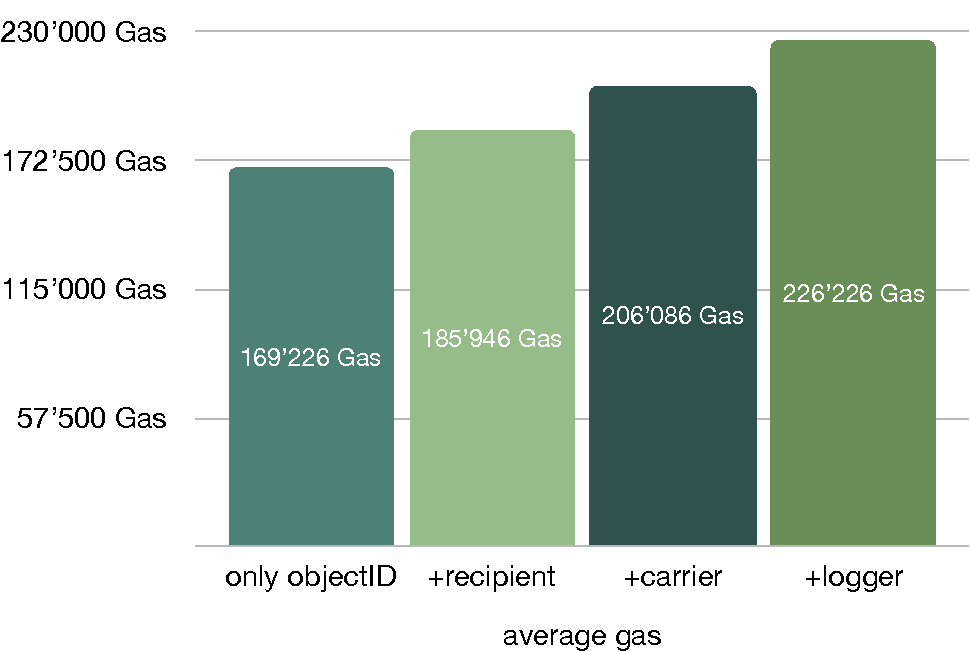
\includegraphics[width=\textwidth]{diagrams/safeMint_gas_eval.pdf}
        \caption{Transaction gas usage}
        \label{fig:safemint_tx_cost}
    \end{subfigure}
    \hfill
    \begin{subfigure}{0.49\textwidth}
        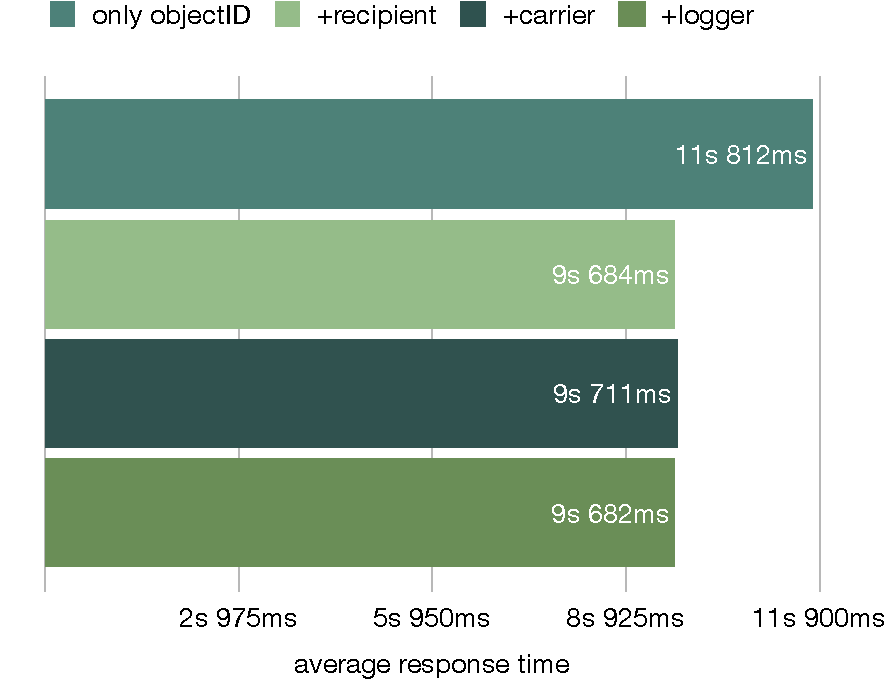
\includegraphics[width=\textwidth]{diagrams/safeMint_request_time_eval.pdf}
        \caption{Request speed in seconds}
        \label{fig:safemint_tx_speed}
    \end{subfigure}
    \caption{safeMint analysis}
    \label{fig:safemint_analysis}
\end{figure}

\subsection*{safeMint}
Figure \ref{fig:safemint_tx_cost} shows the average gas consumed by the safeMint function for a variety of input parameters. Each bar shows the average of 10 function executions. The very left bar shows the average gas used if only the objectID of the artwork is added during minting. The second bar shows the gas consumed if the objectID and the recipient address are provided during minting. This pattern remains the same for the last two bars. The analysis shows that the more parameters are provided the more gas it consumes.

To get a sense of how gas translates into fees we used the average gas price of the past month for the Ethereum mainnet (28 Gwei) \cite{gaspriceaverage} and the current value of Ether in \gls{chf} (1599.32 CHF = 1 ETH) \cite{coinmarketcap}. The results are listed in Table \ref{tab:safemint_tx_fees}. The results show that each artwork \gls{nft} minted costs between 7.71 \gls{chf} and 10.31 \gls{chf}.  

\begin{table}[h]
\begin{tabular}{cllll}
                                          & \textbf{only objectID} & \textbf{+recipient} & \textbf{+carrier} & \textbf{+logger} \\ \cline{2-5} 
\multirow{2}{*}{\textbf{Transaction fee}} & 0.0048 ETH             & 0.0053 ETH          & 0.0059 ETH        & 0.0064 ETH       \\
                                          & 7.71 CHF               & 8.47 CHF            & 9.39 CHF          & 10.31 CHF       
\end{tabular}
\caption{Estimated transaction fees for safeMint}
\label{tab:safemint_tx_fees}
\end{table}

The reponse time of the \gls{api} calls are mostly below 10s. We were not able to observe a large difference when it comes to the different input parameters. The chart in Figure \ref{fig:safemint_tx_speed} shows the average response time in seconds. The maximum response time recorded was 33s on the fifth call with only the objectID submitted and the minimum was 3s with the objectID and recipient address submitted. This shows that this metric can fluctuate heavily depending on the state of the network.

\subsection*{updateArtworkData}
\begin{figure}[h!]
    \begin{subfigure}{0.49\textwidth}
        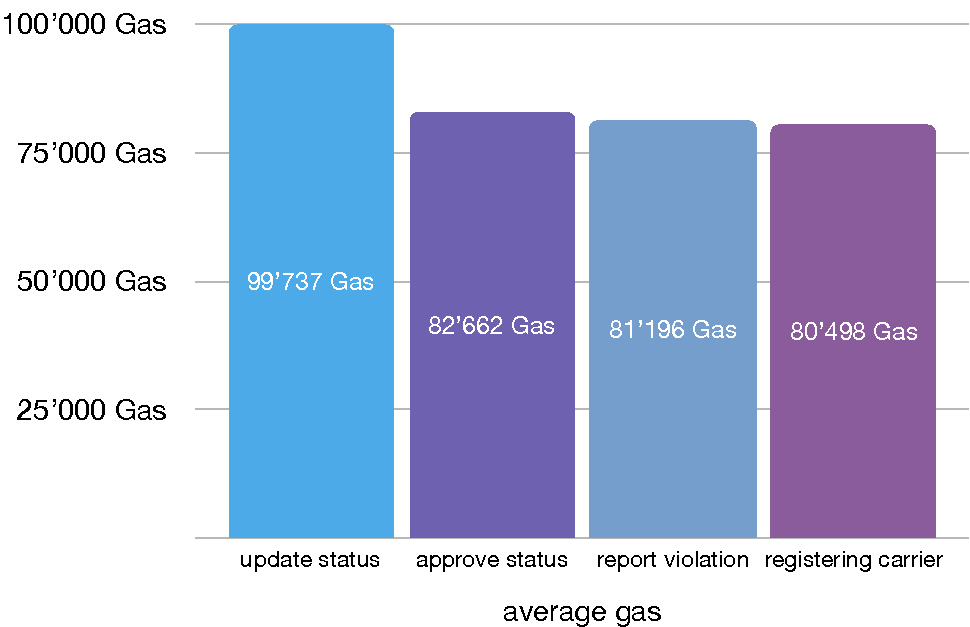
\includegraphics[width=\textwidth]{diagrams/updateArtworkData_gas_eval.pdf}
        \caption{Transaction gas usage}
        \label{fig:updateArtworkData_tx_cost}
    \end{subfigure}
    \hfill
    \begin{subfigure}{0.49\textwidth}
        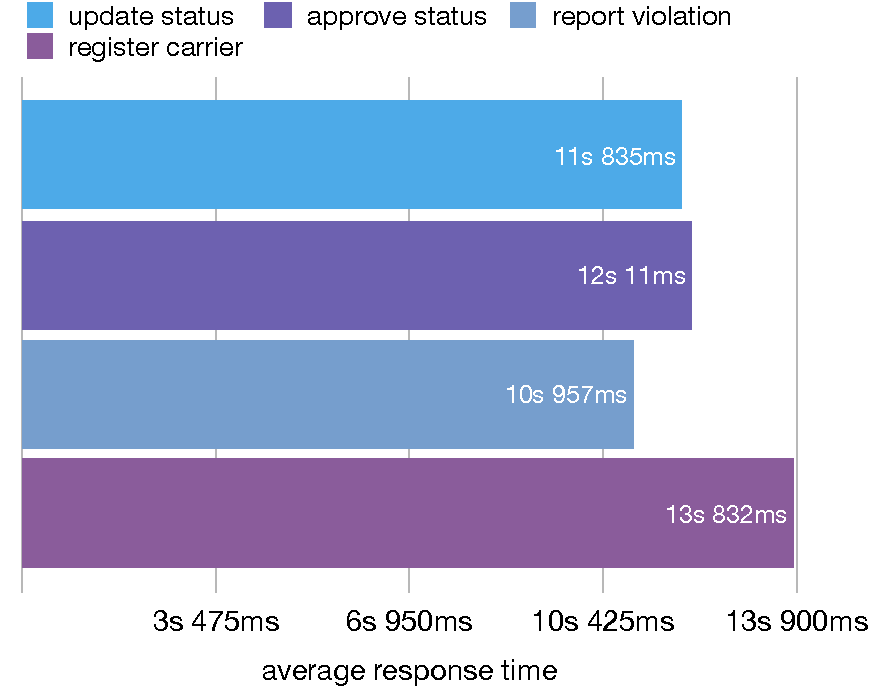
\includegraphics[width=\textwidth]{diagrams/updateArtworkData_request_time_eval.pdf}
        \caption{Request speed in seconds}
        \label{fig:updateArtworkData_tx_speed}
    \end{subfigure}
    \caption{updateArtworkData analysis}
    \label{fig:updateArtworkData_analysis}
\end{figure}

Similarly, we also conducted an analysis of the updateArtworkData function. The bar on the very left of Figure \ref{fig:updateArtworkData_tx_cost} shows the average gas consumed by the function when updating the requested status. Approving the status as a different actor then shows an average gas consumption of 82'662. The last two bars show the gas amount for reporting a violation from the logger and registering a carrier respectively.

The cost of these transactions was estimated in the same manner as with the safeMint function (Table \ref{tab:updateArtworkData_tx_fees}). The results show that updating an artwork \gls{nft} is much less costly than minting it. 

\begin{table}[ht]
\begin{tabular}{cllll}
                                          & \textbf{update status} & \textbf{approve status} & \textbf{report violation} & \textbf{register carrier} \\ \cline{2-5} 
\multirow{2}{*}{\textbf{Transaction fee}} & 0.0028 ETH             & 0.0024 ETH          & 0.0023 ETH        & 0.0023 ETH       \\
                                          & 4.54 CHF               & 3.77 CHF            & 3.70 CHF          & 3.67 CHF       
\end{tabular}
\caption{Estimated transaction fees for updateArtworkData}
\label{tab:updateArtworkData_tx_fees}
\end{table}

The average response time of updating an \gls{nft} vary depending on the input parameters. The request which was fulfilled the fasted was approving a status change with around three Seconds. Interestingly, the longest response time of over 35 seconds was recorded on the same type of request.


\subsection*{Non-Mutating Functions}
The GET endpoints exposed by the \gls{api} target several functions that do not mutate the state of the \gls{sc}. These functions do not cost any gas and their execution time is much less (usually < 1 Second). Additionally, the artis-server adds a caching layer to these function calls which generally reduce the response time of repeated calls to a few milliseconds. 

\section{Field Test}
\label{sec:field_test}
Because the isolated analyses performed above do not indicate how the system would perform during an artwork transportation scenario, we used the system on a simulated transportation scenario. The steps of the simulated scenario are visualized in Figure \ref{fig:eval_scenario} and described in more detail below.

\begin{figure}
    \centering
    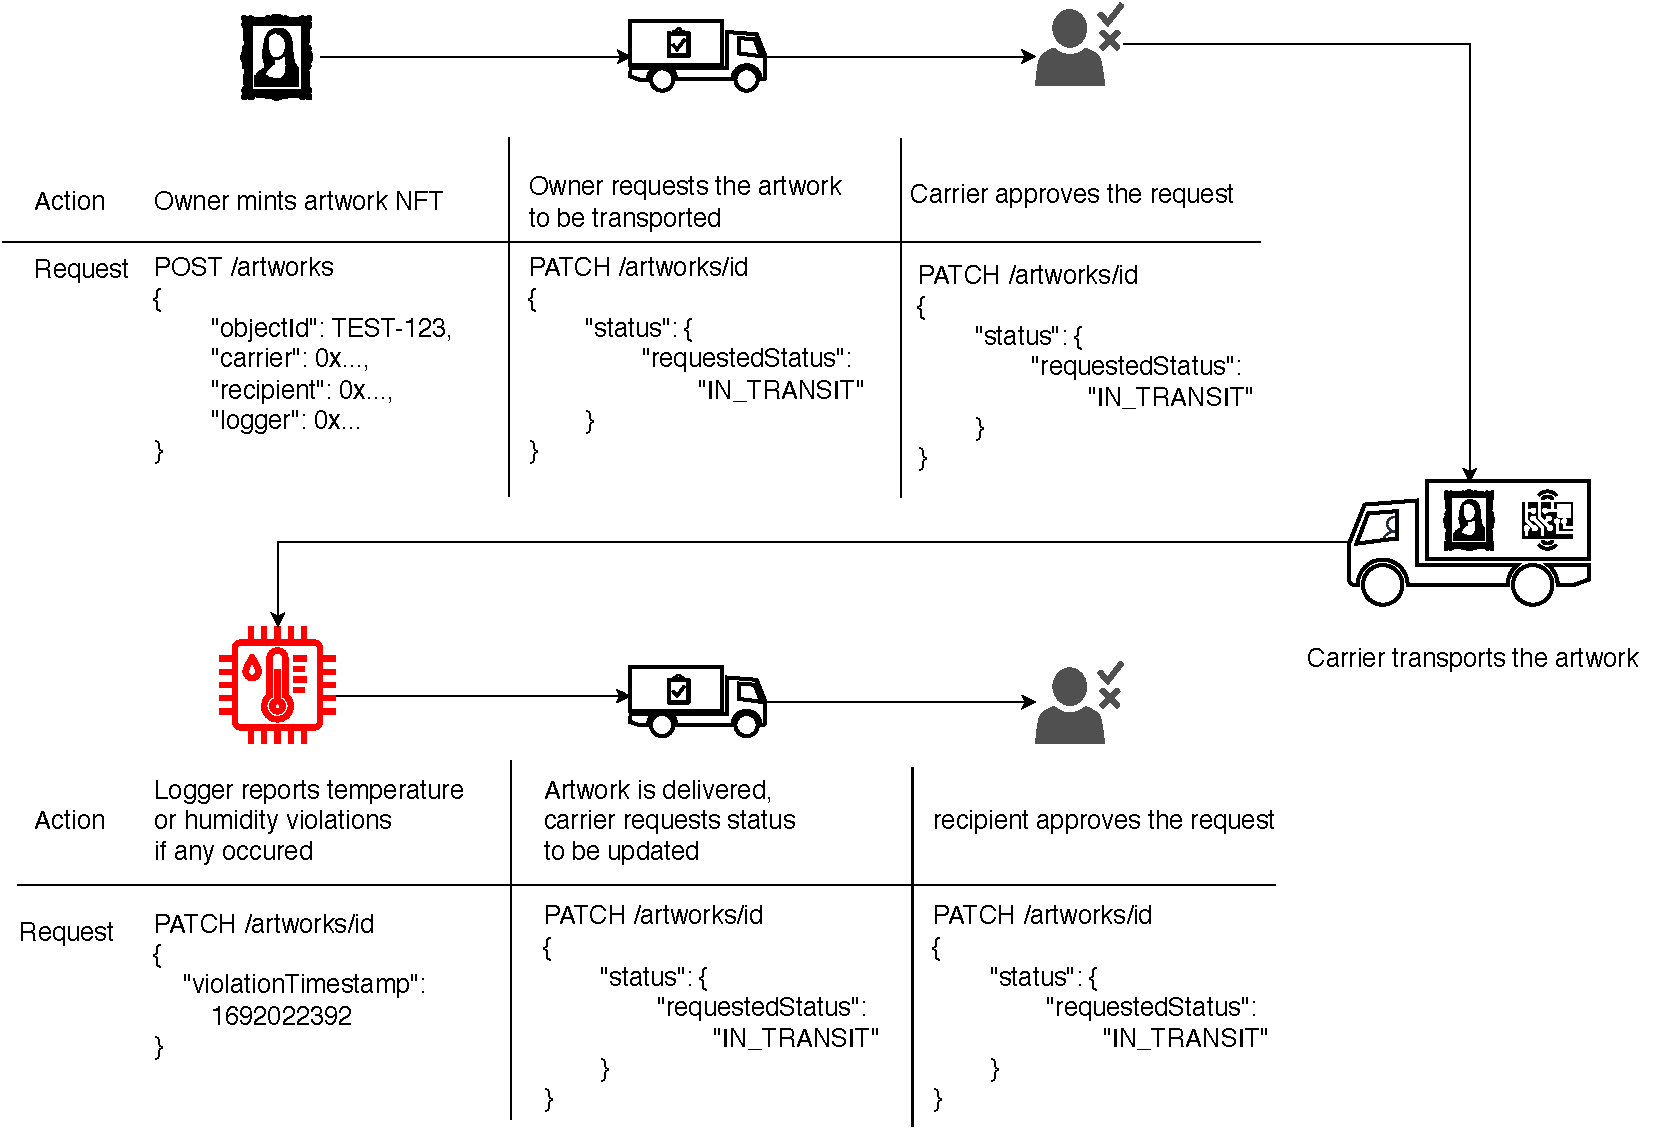
\includegraphics[width=\textwidth]{diagrams/evaluation_scenario_v2.drawio.pdf}
    \caption{Caption}
    \label{fig:eval_scenario}
\end{figure}

The field test involves a minimum of five requests to the \gls{api}. If any violations occur this number is increased accordingly. In our field test we simulated a temperature violation by covering the sensor with our hand (Figure \ref{fig:cover_sensor}).

\begin{enumerate}
    \item create a new artwork \gls{nft} and register the corresponding roles using the artis-frontend.
    \item request the status of the artwork to be changed to \textit{IN\_TRANSIT} from the sender account
    \item approve this request from the carrier account
    \item enable the logger by starting the \textit{logging\_script} and the \textit{violation\_script} with the thresholds of 27 degrees Celcius and 70\% humidity.
    \item take the logging device and transport it from point of departure to destination
    \item during the transportation simulate a violation by wrapping a hand around the sensor to increase the temperature.
    \item upon arrival request the status of the artwork to be changed to \textit{DELIVERED} from the carrier account
    \item approve this request from the recipient account
\end{enumerate}

\begin{figure}[h!]
    \begin{subfigure}{0.5\textwidth}
        \centering
        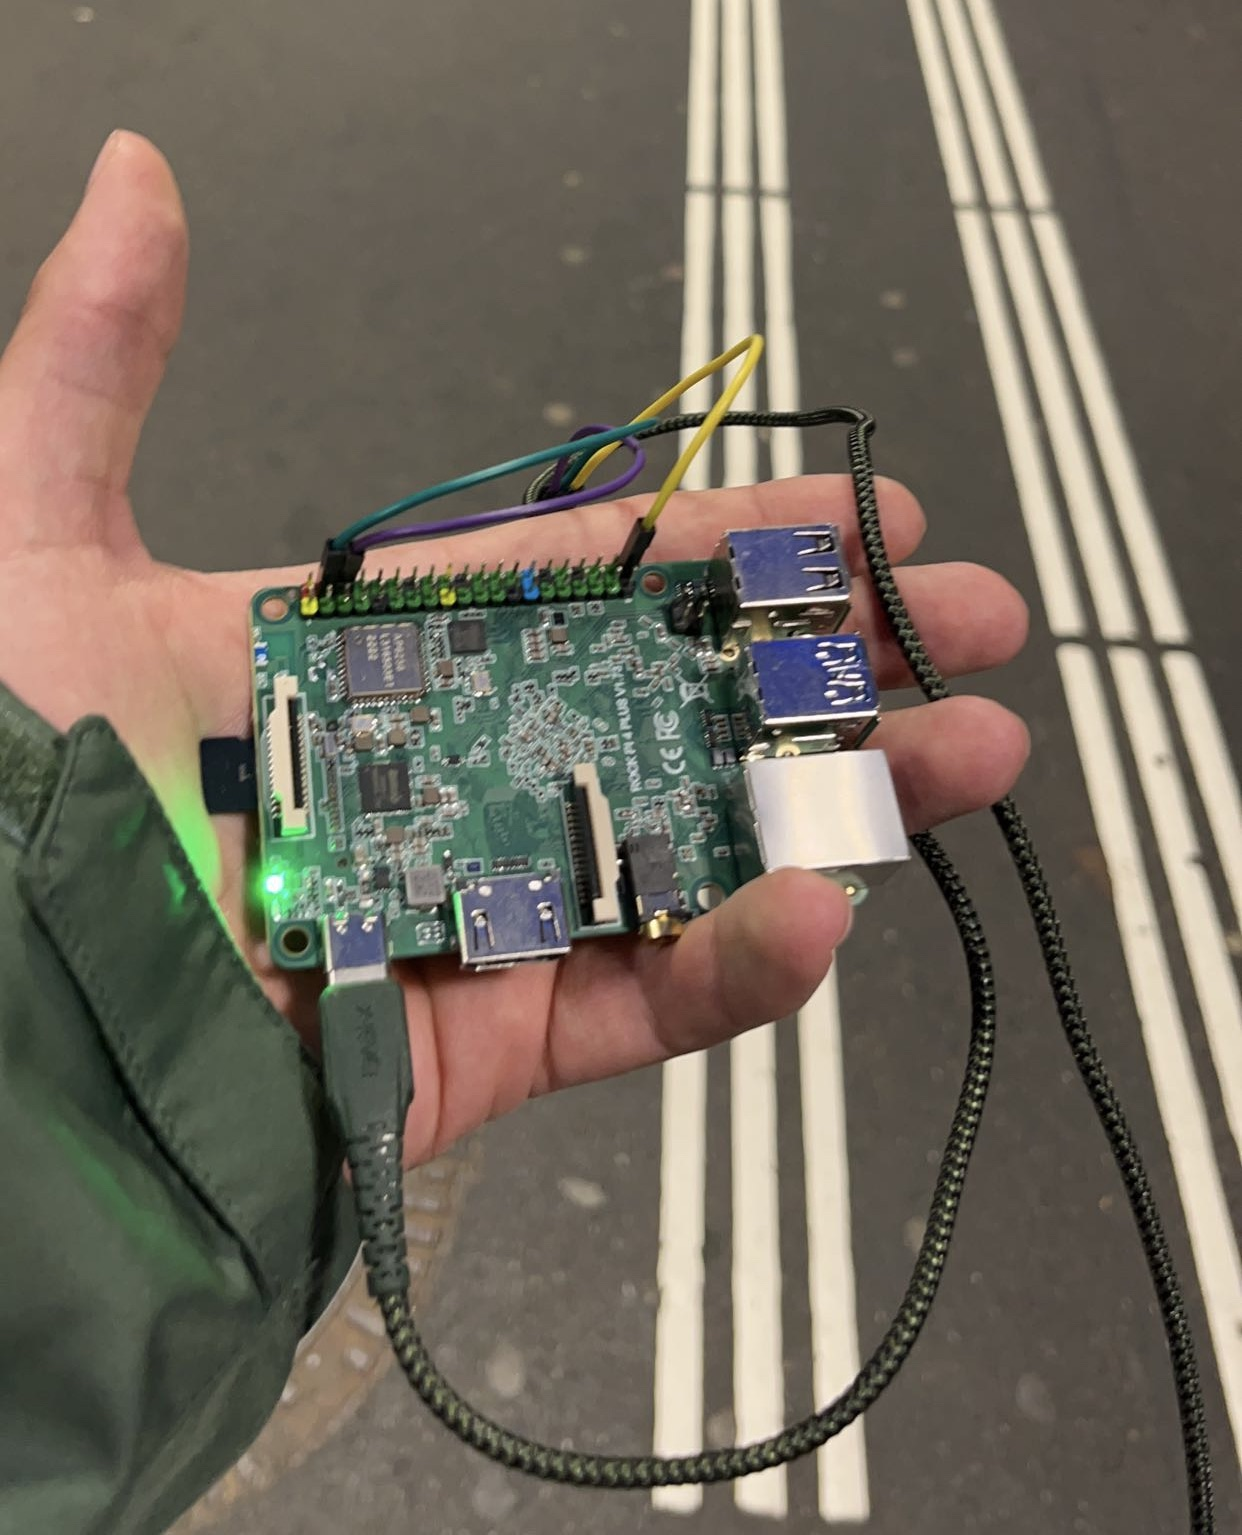
\includegraphics[height=0.25\textheight]{resources/field_test.jpeg}
        \caption{Simulating artwork transportation scenario}
        \label{fig:sensor_transport}
    \end{subfigure}
    \hfill
    \begin{subfigure}{0.5\textwidth}
        \centering 
        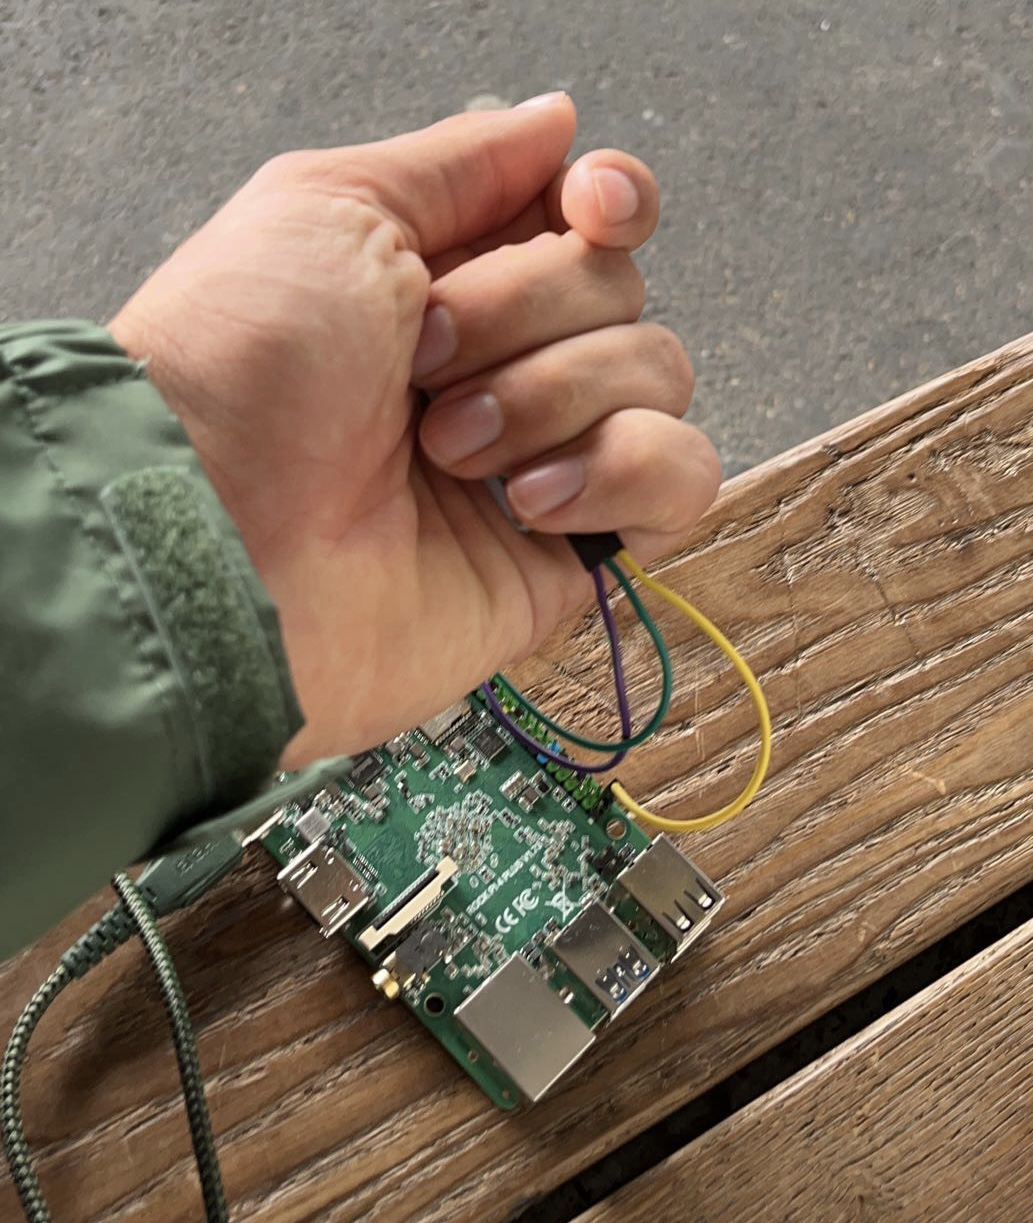
\includegraphics[height=0.25\textheight]{resources/cover_sensor.jpeg}
        \caption{Simulating temperature violation}
        \label{fig:covering sensor}
    \end{subfigure}
    \caption{System Field Test}
    \label{fig:field_test}
\end{figure}


\subsection{Cost}
\subsection{Logger performance}


\section{Discussion}
\label{sec:eval_discussion}